\tableofcontents
\newpage

% ======= Constancias y Reconocimientos =======
\phantomsection
\addcontentsline{toc}{section}{Constancias y Reconocimientos}

\phantomsection
\addcontentsline{toc}{subsection}{Constancia Verano Científico OAN}
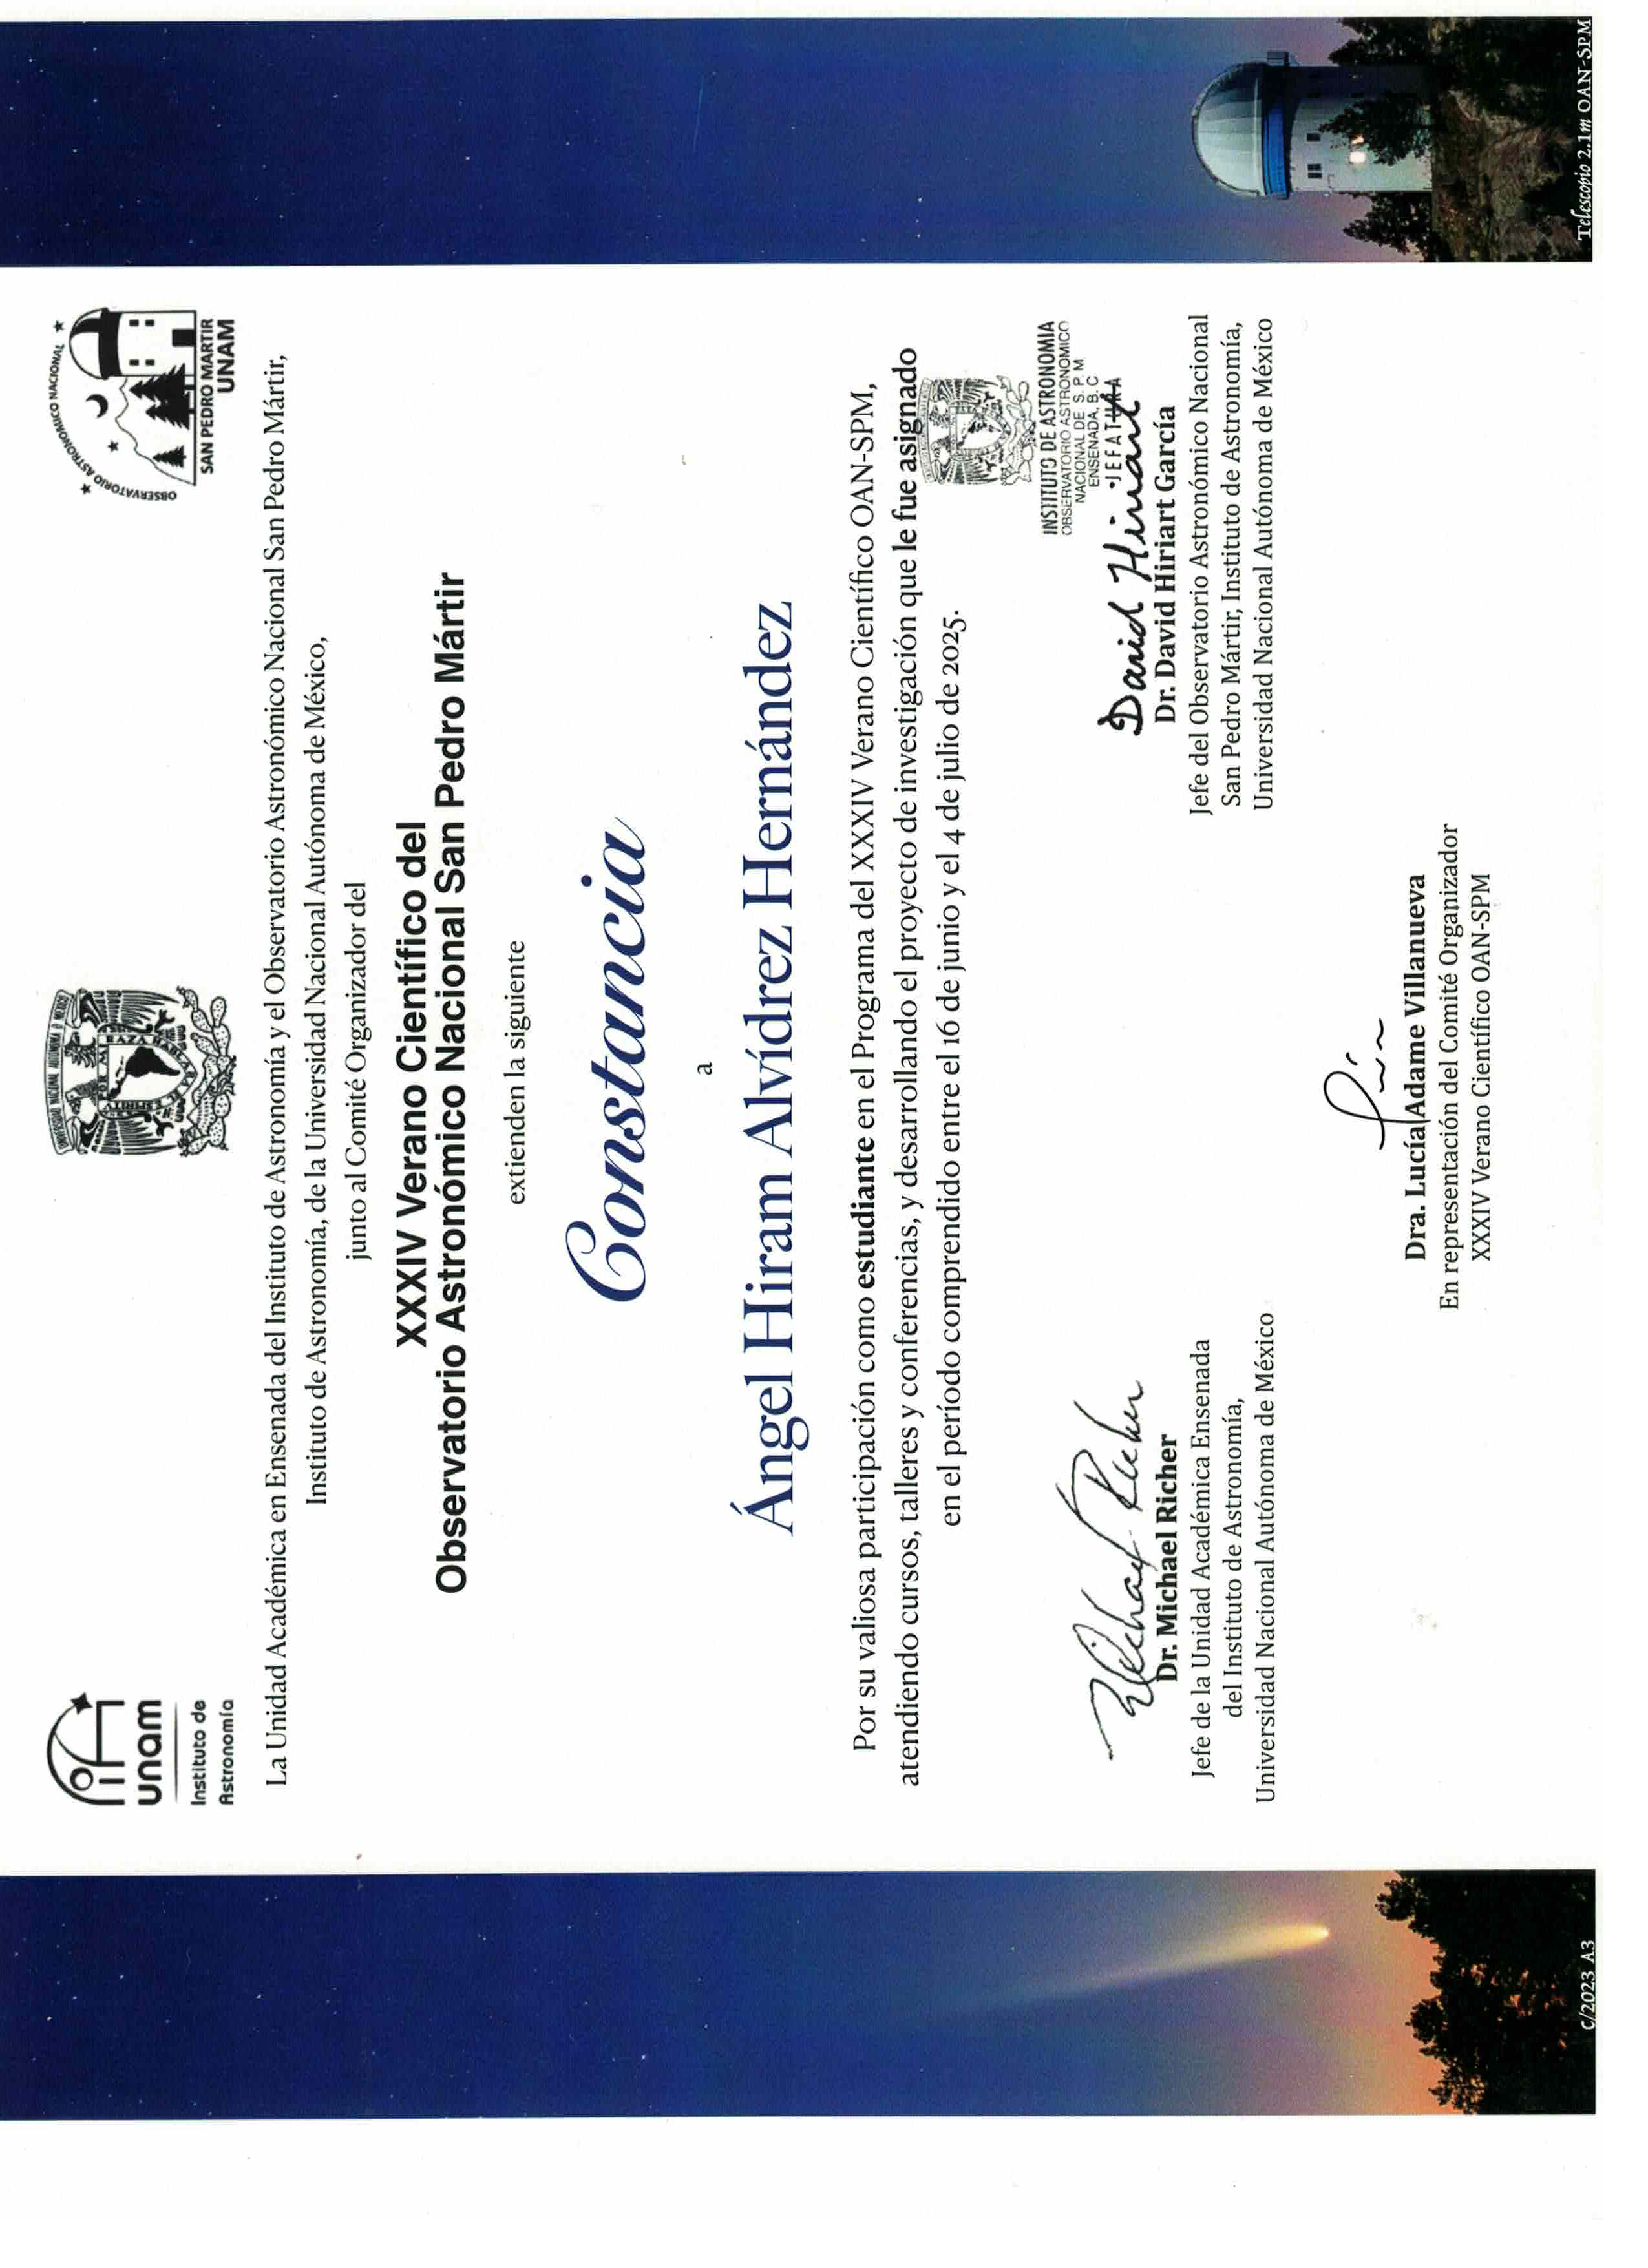
\includepdf[pages=-]{ConstanciaOAN.png}

\phantomsection
\addcontentsline{toc}{subsection}{Constancia Fundamentos de Semiconductores}

\includepdf[pages=-]{ConstanciaSemiconductores.png}

\phantomsection
\addcontentsline{toc}{subsection}{Reconocimiento Como Estudiante Integral}
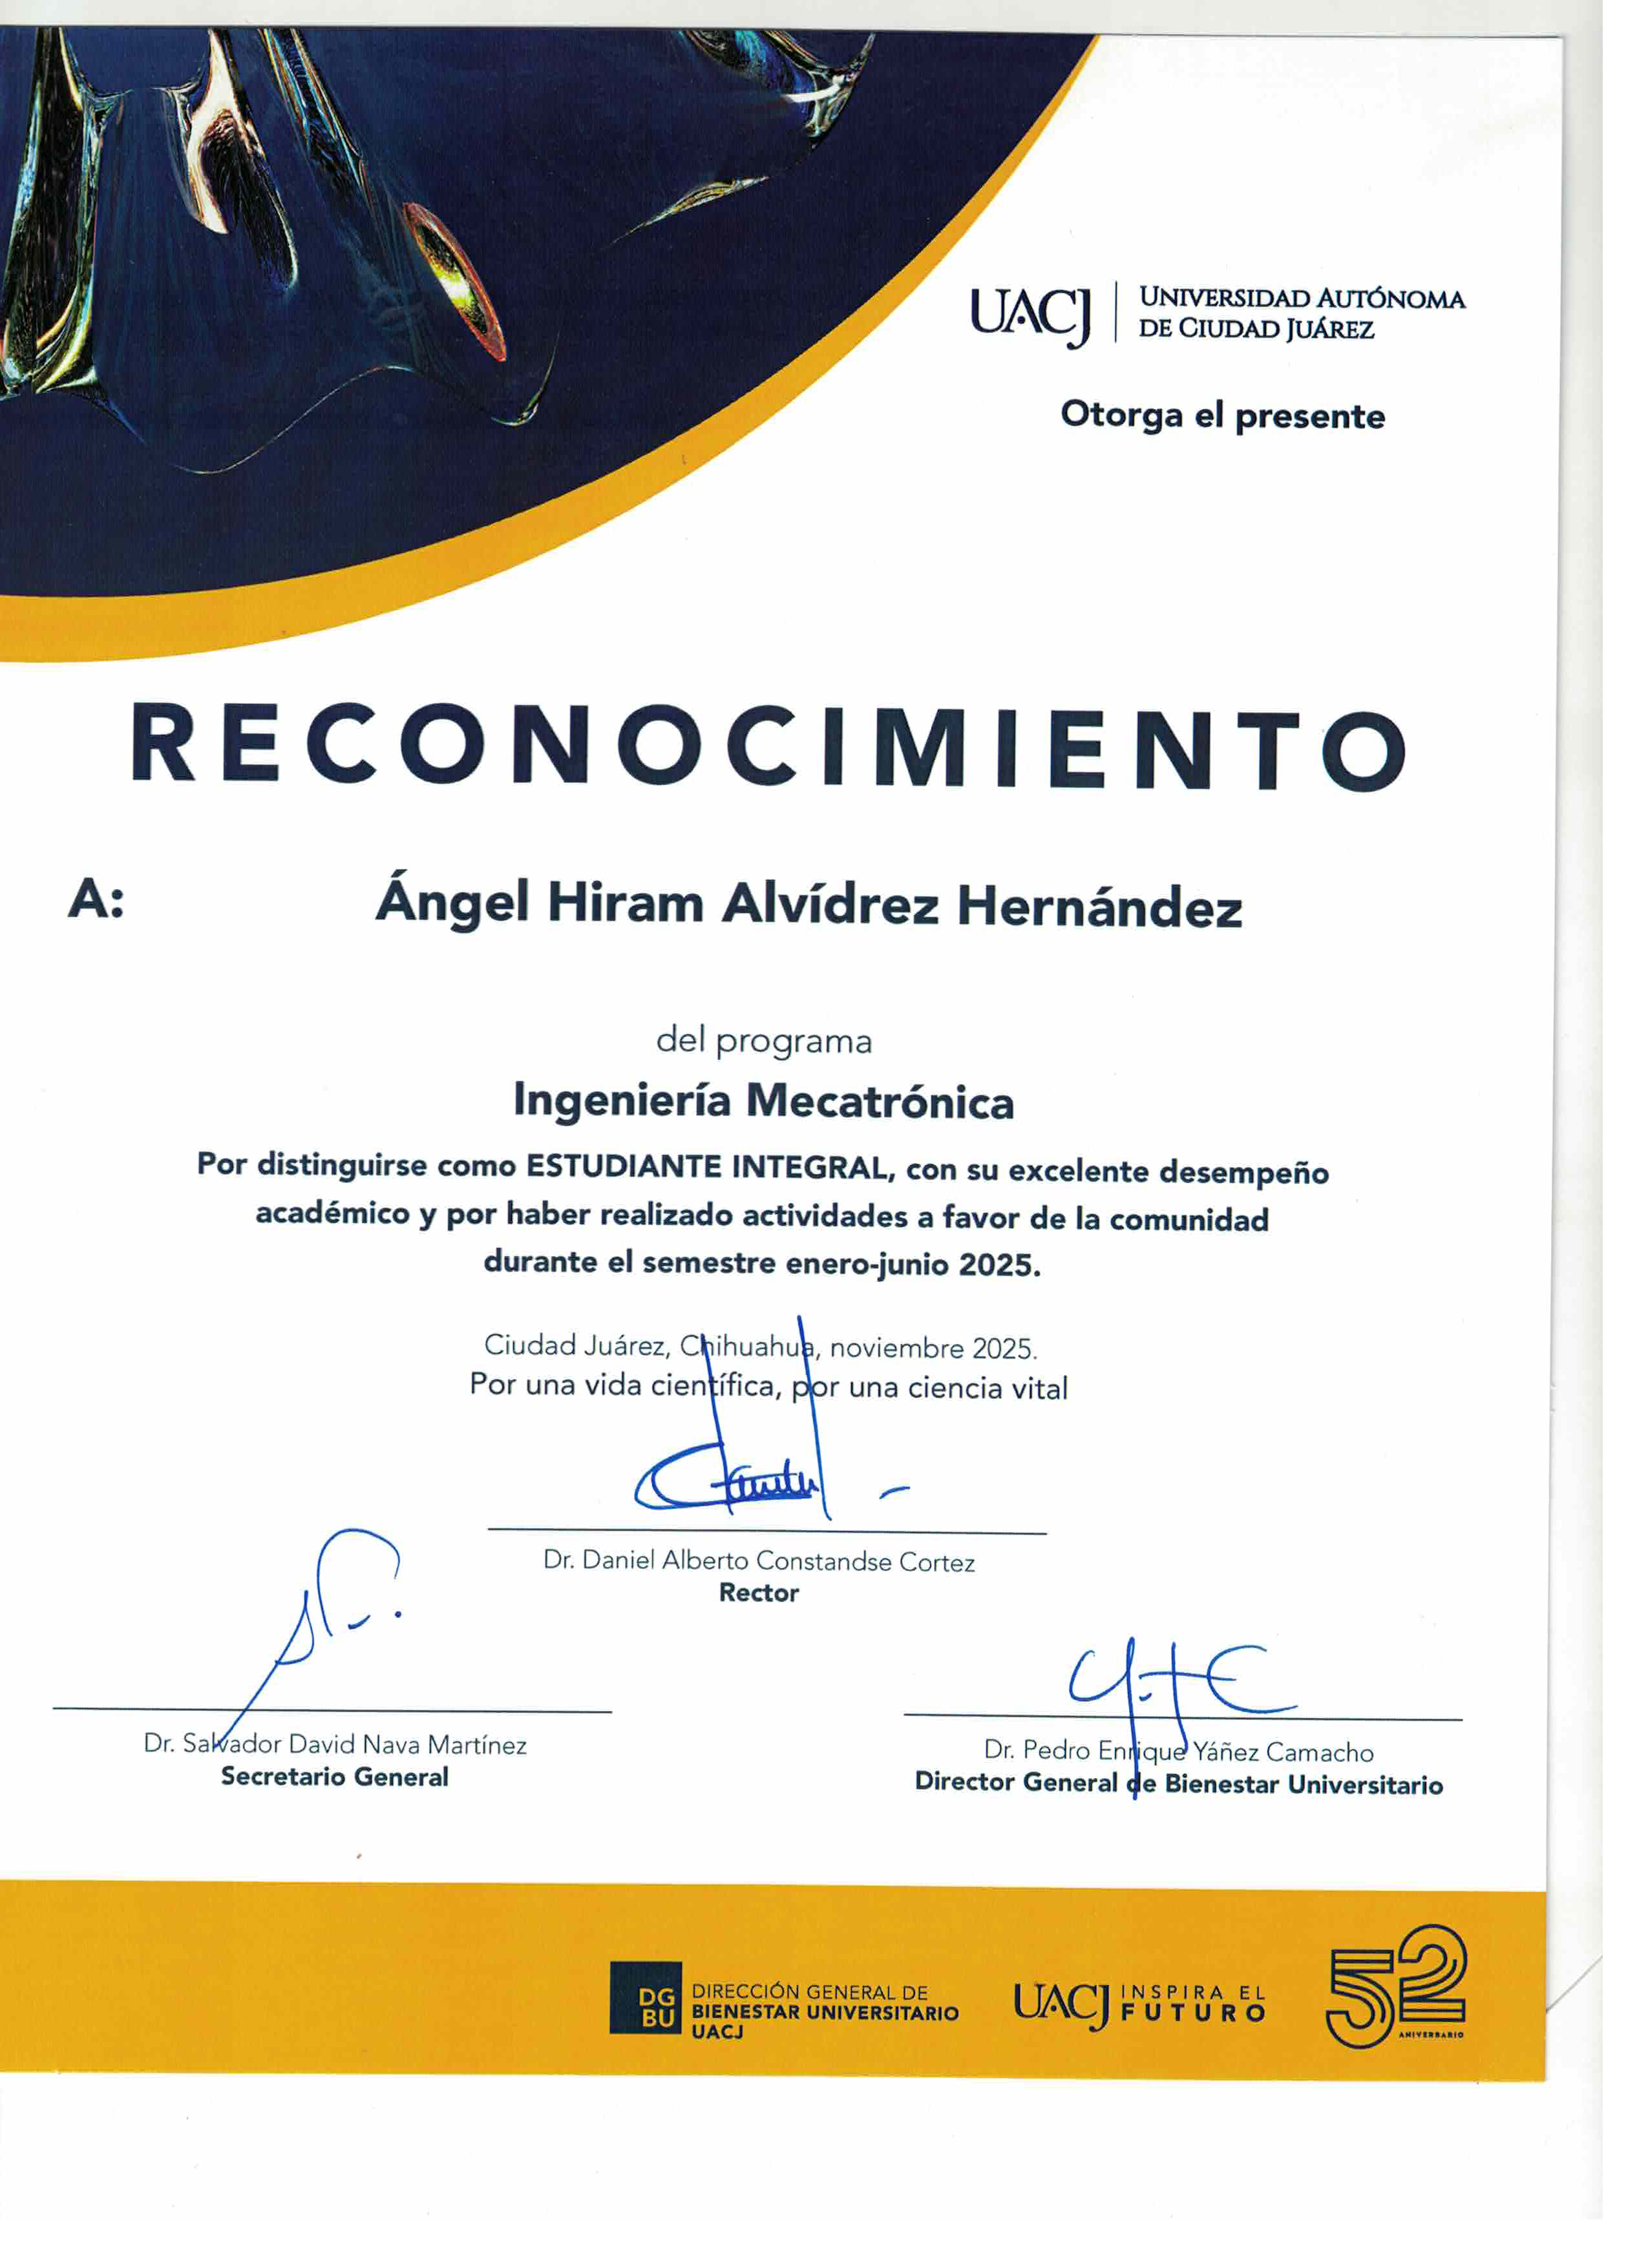
\includepdf[pages=-]{ReconocimientoEstudianteIntegral.png}

\phantomsection
\addcontentsline{toc}{subsection}{Reconocimiento por Impartir conferencia: Realmente Estamos solos en el universo?}
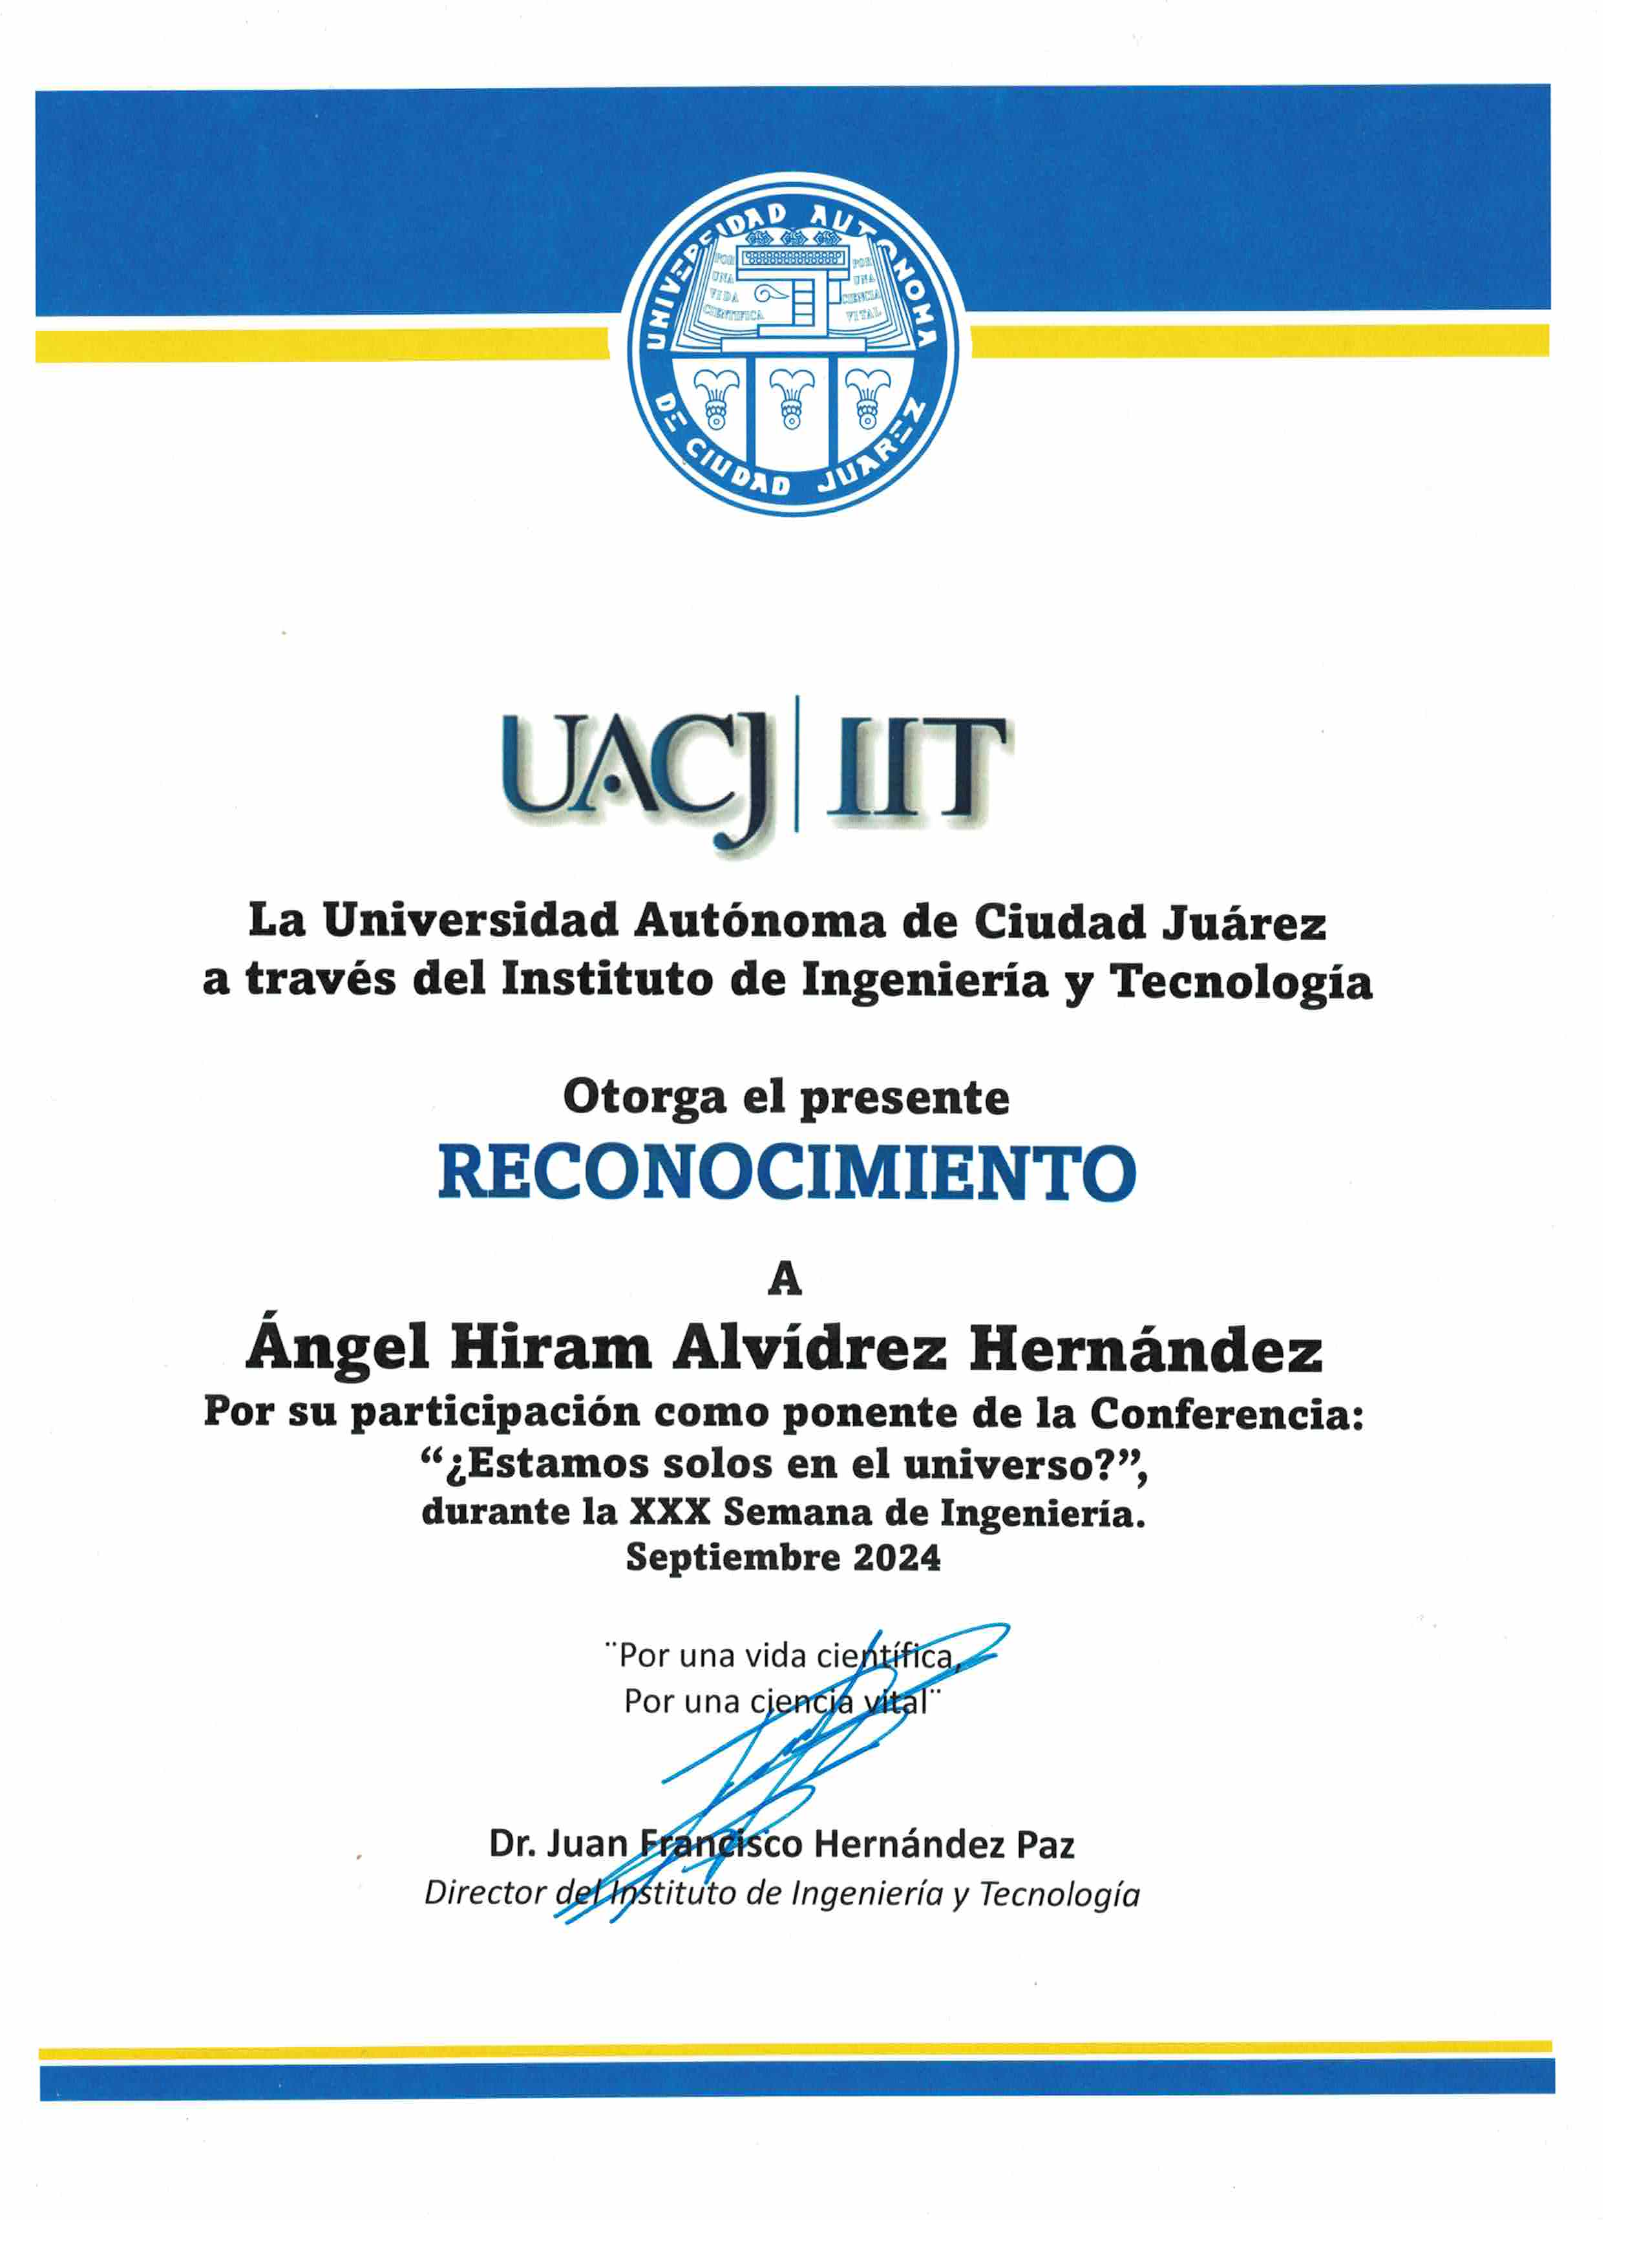
\includepdf[pages=-]{ReconocimientoConfSolosUniverso.png}

\phantomsection
\addcontentsline{toc}{subsection}{Reconocimiento por Impartir conferencia: Las muertes del Universo}

\includepdf[pages=-]{ReconocimientoConfMuertesUniverso.png}

% ======= Proyectos y Prácticas de Ingeniería =======
\phantomsection
\addcontentsline{toc}{section}{Proyectos y Prácticas de Ingeniería}

\phantomsection
\addcontentsline{toc}{subsection}{Bípedo subactuado Basado en un Mecanismo de 5 Barras}
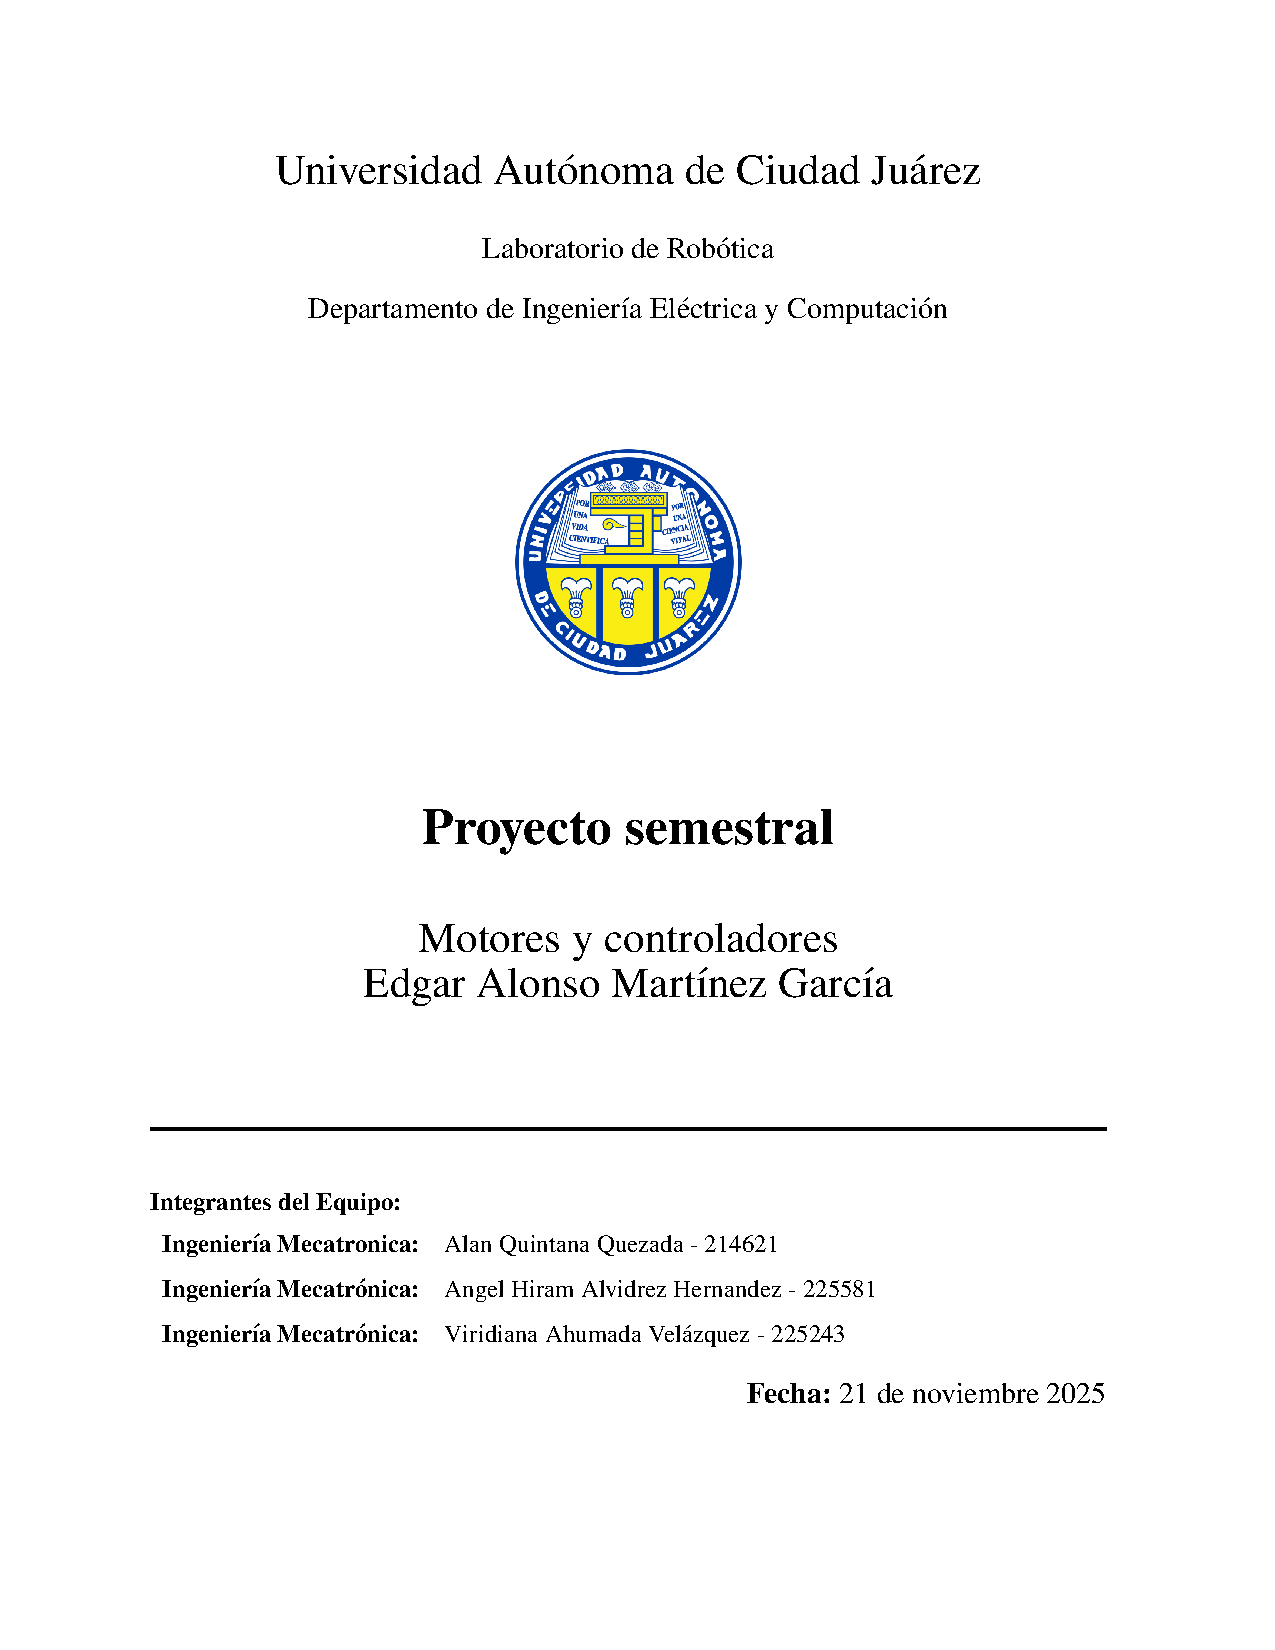
\includepdf[pages=-]{ProyectoSemestral_MotoresyControladores.pdf}

\phantomsection
\addcontentsline{toc}{subsection}{Actualizacón de la Electrónica de Control de un Telescopio}
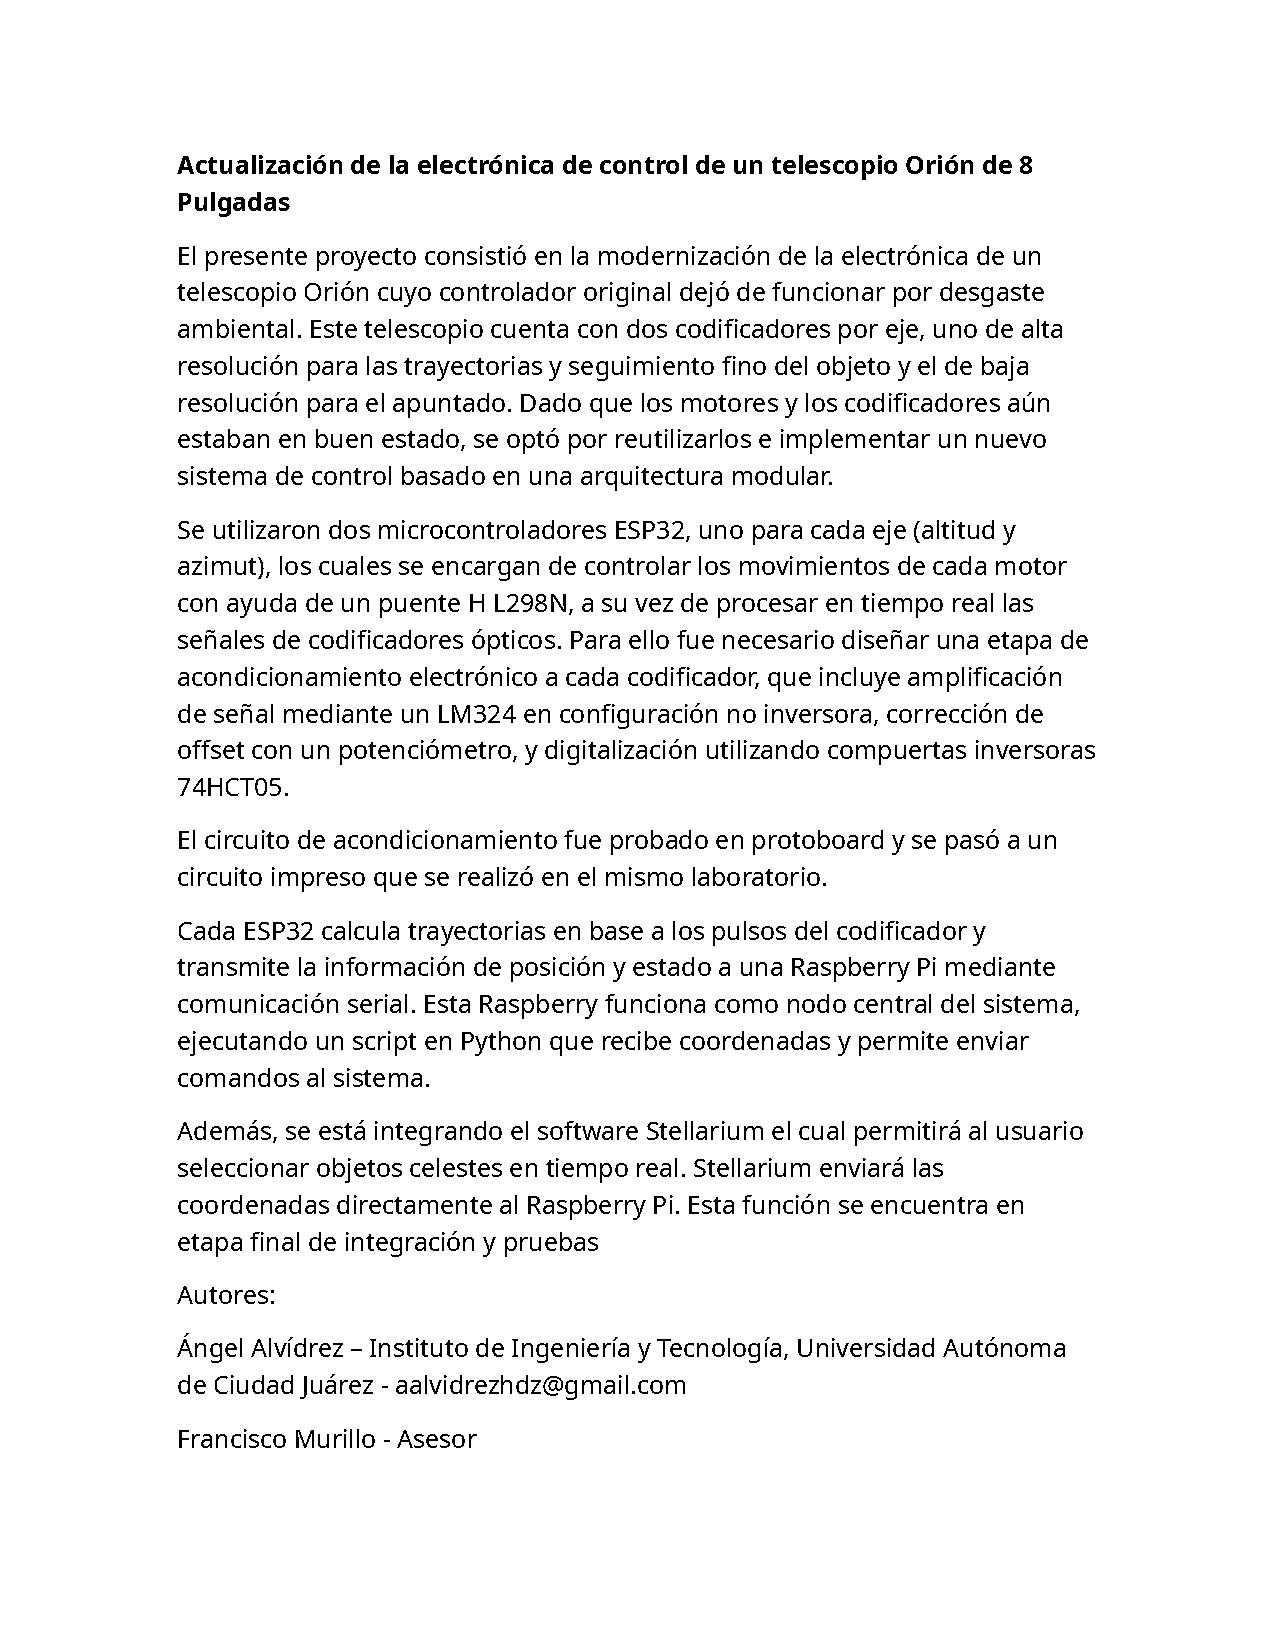
\includepdf[pages=-]{telescopio.pdf}


\phantomsection
\addcontentsline{toc}{subsection}{Amplificador de Guitarra mediante Transistores}
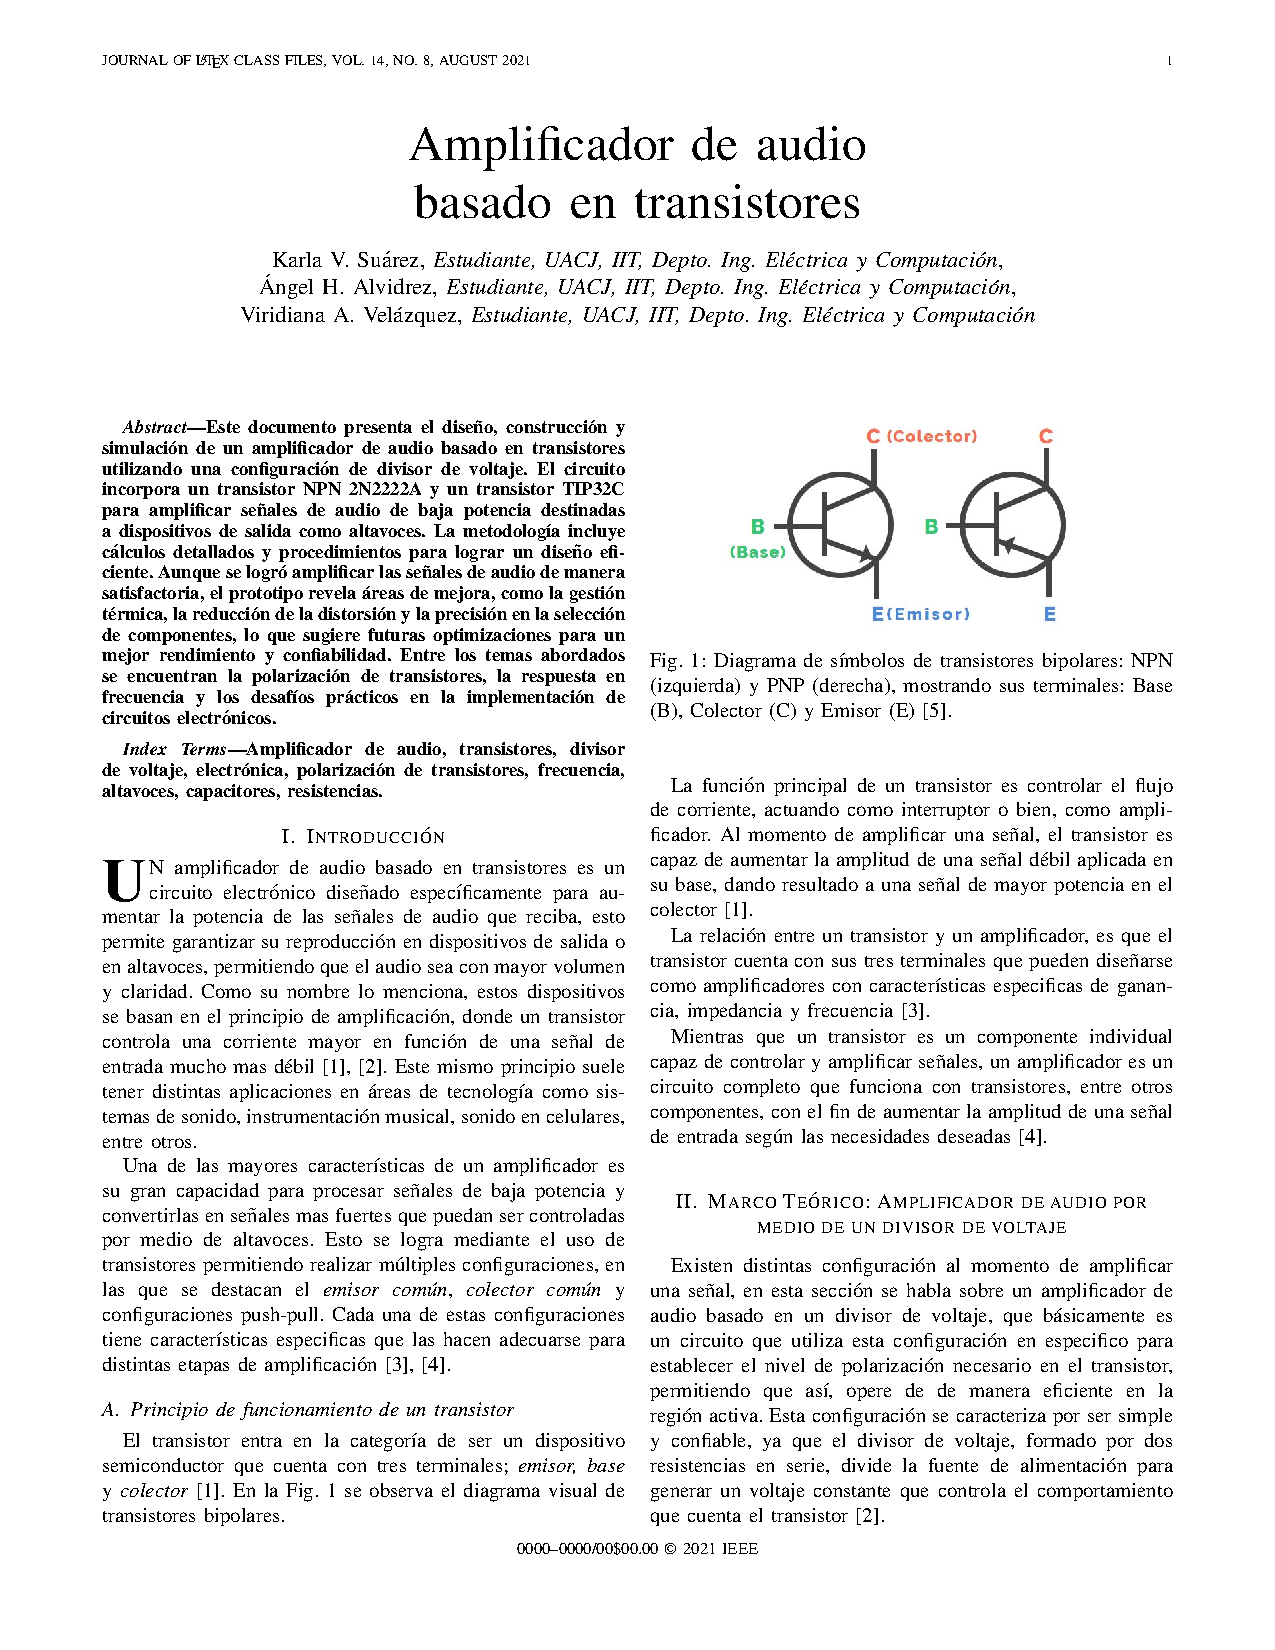
\includepdf[pages=-]{amplificador.pdf}

\phantomsection
\addcontentsline{toc}{subsection}{Control de Posición de un carrito con PID}

\includepdf[pages=-]{Control_de_Posicion_Carrito_PID.pdf}

\phantomsection
\addcontentsline{toc}{subsection}{Carrito Seguidor de Líneas}

\includepdf[pages=-]{Carrito_Seugidor_de_lineas.pdf}

\phantomsection
\addcontentsline{toc}{subsection}{Encendido y Apagado de un Foco con Aplausos}

\includepdf[pages=-]{Sensor_De_Aplausos_Apagado_Prendido_Foco.pdf}

\phantomsection
\addcontentsline{toc}{subsection}{Sistema de Riego IoT (ESP32 + Blynk)}
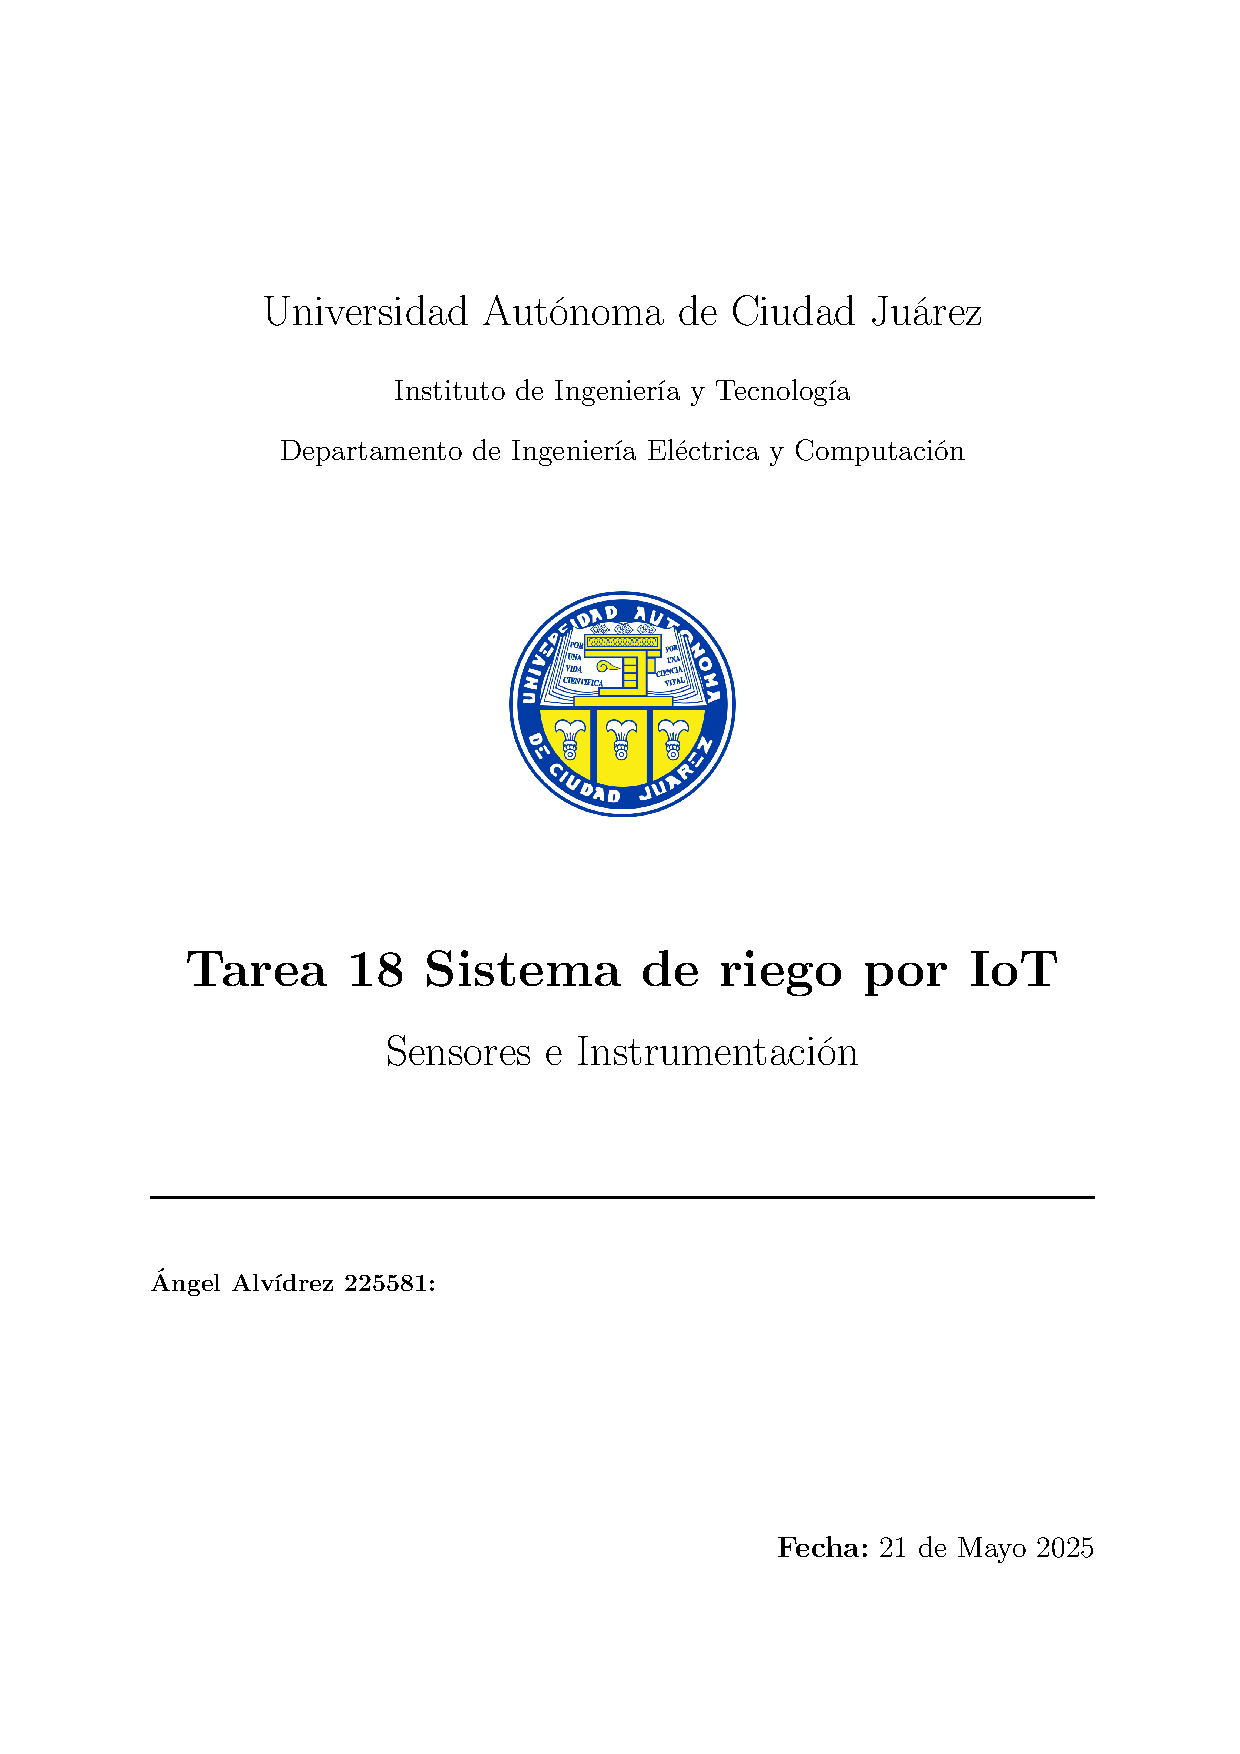
\includepdf[pages=-]{Sistema_De_Riego_IOT.pdf}

% ======= Publicaciones y Trabajos Académicos =======
\newpage
\phantomsection
\addcontentsline{toc}{section}{Publicaciones y Trabajos Académicos}

\section*{Publicaciones y Trabajos Académicos}

\phantomsection
\addcontentsline{toc}{subsection}{Artículo en revisión: Kinematic Modelling of Five-Bar Bipedal Locomotion}

\subsection*{Artículo en revisión: Kinematic Modelling of Five-Bar Bipedal Locomotion}

\textbf{Kinematic Modelling of Five-Bar Bipedal Locomotion: An Analytical Approach}

\vspace{0.3cm}

\textit{Estado: En revisión (Under Review)}

\textit{Conferencia: 30th International Conference on Methods and Models in Automation and Robotics (MMAR 2026)}

\textit{Submission ID: 3077}

\vspace{0.3cm}

\textbf{Autores:} Ángel H. Alvídrez-Hernández, Edgar A. Martínez-García

\vspace{0.5cm}

\textbf{Descripción:}

Este trabajo presenta un modelo analítico para la cinemática de un robot bípedo basado en un mecanismo de cinco barras. 
Se desarrollan las ecuaciones de cinemática directa e inversa, así como un mapeo determinístico entre el espacio de articulaciones 
y el espacio de tarea. Además, se implementa un filtro de Kalman para la estimación del estado del sistema, permitiendo el seguimiento 
de trayectorias y la estabilización del movimiento en un prototipo experimental.

\vspace{0.7cm}

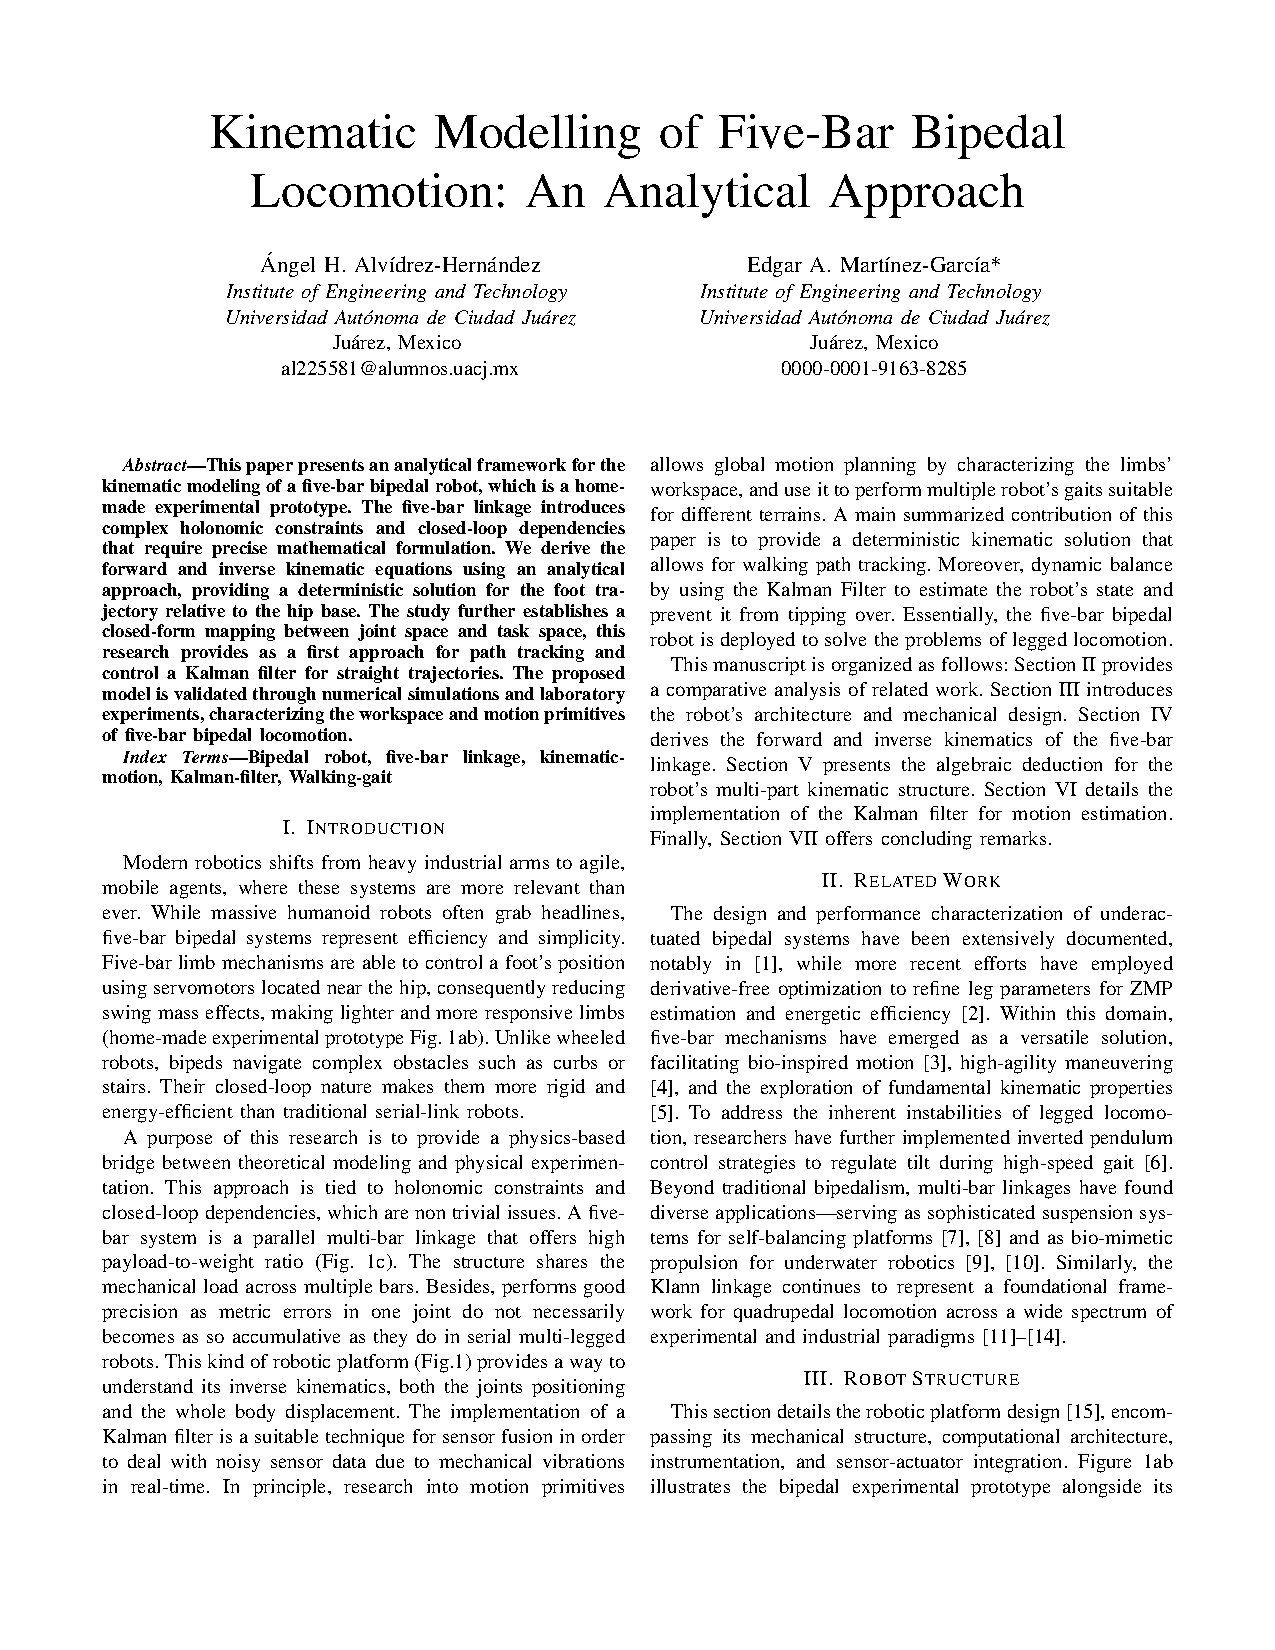
\includepdf[pages=-]{MMAR26_confBiped5b.pdf}